\documentclass[english,12pt]{article}
\usepackage[T1]{fontenc}
\usepackage{geometry}
\geometry{verbose,bmargin=2.5cm,lmargin=2.5cm,rmargin=2.5cm}
\usepackage[utf8]{inputenc}
\usepackage{amsmath}
\usepackage{amsfonts}
\usepackage{amssymb}
\usepackage{rotfloat}
\usepackage{wasysym}
\usepackage{graphicx}
\usepackage{natbib}
\usepackage{latexsym}
\usepackage{caption}
\usepackage{flafter}
\usepackage{babel}
\usepackage{imakeidx}
\usepackage{amssymb,amsmath}
\usepackage[table]{xcolor}
\usepackage[mathlines,displaymath]{}
\usepackage{anyfontsize}
\usepackage{verbatim}

\newcommand{\etal}{{et~al.{}}}
\newcommand{\ie}{{i.~e.{}}}
\newcommand{\eg}{{e.~g.{}}}
\newcommand{\viz}{{viz.{}}}
\newcommand{\etc}{{etc.{}}}
\newcommand{\apriori}{{a priori{}}}
\newcommand{\vv}{{vice versa{}}}
\newcommand{\cf}{{}}
\usepackage{titling}
\usepackage{color}
\usepackage{subfigure} 

\date{}

\topmargin 0.0cm
\oddsidemargin 0.5cm
\evensidemargin 0.5cm
\textwidth 16cm 
\textheight 22cm

\makeindex
\begin{document}
\begin{flushleft}
  \textbf{\Large Automated research platforms}\\
Ali R. Vahdati\textsuperscript{1, *}\\
Charles N. de Santana\textsuperscript{2}\\
Alejandro Rozenfeld\textsuperscript{3}\\
Carlos J. Meli\'an\textsuperscript{4, *}\\
  \vspace{0.5cm} 
\textbf{1} Department of Anthropology, University of Zurich, Switzerland\\
\textbf{2} Institute of Evolutionary Biology and Environmental Studies, University of Zurich, Switzerland\\
\textbf{3} Conicet-cificen-intelymec, University of the Center of Buenos Aires, Argentina\\
\textbf{4} Department of Fish Ecology and Evolution, Center for Ecology, Evolution and Biogeochemistry, EAWAG, Kastanienbaum, Switzerland
\\
\bigskip
\end{flushleft}
* These authors contributed equally to this work.\\
\newpage


\tableofcontents
\newpage

\section{Abstract}
High-resolution and heterogeneous data coming from many sources is
standard in science, engineering and investment landscapes. Yet,
automated inference providing insightful patterns and processes
integrating databases with analytical frameworks remains
challenging. In this work we propose a prototype of an automated
research platform to discuss the challenges for automated workflows to
integrate data and pattern-process-based inference accounting for many
sources of uncertainty. Automated research platforms can strongly
contribute to the science of science to take better informed decisions
in research, management and investment landscapes.
\\
\\
Keywords: data integration, multilayer networks, deep process-based
learning, approximate Bayesian computation, inference.
\newpage


\section{Introduction}

Automation is rapidly occurring in many fronts, from robotics and
investments to gaming and ecommerce. What about science? Science is in
a era of massive data accumulation, integration and pattern
detection. Yet, obtaining insights from such an integration accounting
for reproducibility, inference and prediction power is at a very
incipient stage \citep{Ioannidis2005,Reichsteietal2019}. There are
many challenges when aiming to integrate data, inference and
prediction. For example, sampling design and experiments \index{robust
  experiments} \citep{Voelkl2018}, randomizations to achieve solid
statistics \index{robust algorithms}, and process- or pattern-based
model selection and inference \index{robust inference} just to name a
few require many intermediate decisions that make the scientific
process challenging to repeat, replicate, and reproduce. Currently,
there are many protocols and platforms automatizing partial steps of
the scientific cycle (Table 1). Here, we summarize automated platforms
to analize the existing gaps with the aim to automate the whole
scientific cycle (Figure 1). Open automated research platforms
\index{Open automated research platforms} might play a leading role in
addressing at least the five following challenges: 1) Helping in the
science of science by providing quantitative statistics
\citep{Fortunatoeaao0185}, for example, the many paths with solutions
to specific questions; 2) Identifying systematically bias and
uncertainty in inference; 3) Exploring prediction and explanatory
gradients to gain sinergy between predictive and explanatory power to
complex problems; 4) Identifying gaps in patterns not explored
consequence of lack of syntesis within and between disciplines, and 5)
Allowing for reusability, repeatibility, replicability and
reproducibility along the many paths in the scientific enterprise
(Figure 1).

1. Testing science: Helping select the best paths in responding to a question? ARP can provide a distribution of solutions by classifying the topologies of the multilayer networks. \\
2. Identifying bias and uncertainty in inference. \\
3. Exploring predictions-explanatory gradients to gain sinergy between predictive and explanatory power. \\
4. Identifying gaps in patterns not explored consequence of lack of integration within and between disciplines, and \\
5. Facilitating the 4R in open science: reusability, repeatability, replicability, and reproducibility. \\


The design or research platforms is still in its infancy. Many factors
are involved in research platforms: the programming language, the
number of packages and their interactions, their efficiency and
functionality, etc.


Many questions in science strongly depend on our own bias, lab inertia
in the methods and data explored. Therefore, exploring new paths would
require new efforts to lead to new methods or new collaborations...

Reproducibility and robustness across the different stages of a
research platform are two of the desire properties. Reproducibility
guarantees the future improvement of the results in future
analysis. Many programming languages have tools to facilitate
reproducibility (notebooks) and notebooks implementing many languages
are already available (jupyter...). Automated research platforms track
the explored paths (i.e., the within and between layer interactions)
and outlines how close each path is to the empirical patterns
accounting for

%Robust experiments
Sampling desing and experiments...\\

% Robust algorithms
Randomizations to achieve solid statistics...\\

%Robust inference
One of the most discussed challenges nowadays is how to balance
pattern and process inference. Many problems might not require a
mechanistic understanding to make predictions. Recent examples are AI
algorithms playing chess and go. They do not require a theory of mind
to win. On the other side, there can be problems that might require a
solid mechanistic understanding to make accurate predictions. Examples
of these problems can be global warming or astrophysics. Therefore
platforms that learn to combine AI and process-based methods

%Example and results exploring PI vs TI gradient -- PI, TI or hybrid PTI 


\section{The structure of automated research platforms}
In this section we outline the steps to develop a research
platform. We introduce each of the layers outlined in Figure 1, data
collection and integration (DC), complexity reduction, pattern-process
inference, validation and visualization. The second part introduces a
simple example using the $\mathcal{ROBHOOT}$ package.


For any given question, there are different
methods within each layer that can complete the task. Ideally, one
should be able to choose the best method from each layer and connect
them to reach insightful patterns and predictions from the data. How
many paths are there? Which of these minimize bias? Which topology
within and between layers give the best response to our question?

\subsection{Data Integration}

Data access platforms within and qacross disciplines are highly
scattered across the web
\footnote{\url{https://github.com/melian009/Robhoot/blob/master/resources/databases.md}}. Researchers
have to deal with a highly complex set of intermediate stages and
regulations before having access to the raw data. Having ``easy''
access to the information in a ``perfectly informed market'' should be
simple and efficient, but unfortunately, it is not. Data integration
in research platforms is rapidly evolving and there are many platforms
that can have access and deliver real time data plots (Table 1).

Data Integration and standarization -- Size effects -- N labs vs N
samplings per lab: Accuracy and uncertainty: How do initial
distributions change accuracy and uncertainty? Trade-offs experimental
vs big data

\subsection{Complexity Reduction}

\begin{comment}
PCA family -- High-dimensionality of Convex hull -- Information metrics multilayer networks\\


Data dimension reduction is a second step to increase performance
during the next stages of analysis.  Complexity reduction in economics
and in ecology has a long tradition mostly by looking at
variance-covariance matrices.  Portfolio theory in economics has a
long tradition \citep{MarkowitzBook}. The theory is rooted in the
concept of efficient frontier\index{efficient frontier}. There are
several packages in several languages to calculate efficient
frontiers\footnote{\url{http://www.quantcode.com/}}$^{,}$\footnote{\url{https://github.com/JuliaQuant/PortfolioModels.jl}}$^{,}$\footnote{\url{https://www.wikinvest.com/account/portfolio/register}}$^{,}$\footnote{\url{https://d1so5k0levrfcn.cloudfront.net/SigFig\%20Investment\%20Methodology.pdf}}. Most
maths underlying portfoliio theory\index{portfolio theory} are based
in matrix correlation patterns\index{matrix correlation patterns}. In
ecology, portfolio concept has also been used to predict the number of
coexisting species in landscapes with highly fluctuating
environments\footnote{Check references}.

Many fields aim at predicting fluctuations of several time series at
local and regional scales. The better the predictions are the better
we know the ecosystem. Unfortunately, it is not easy to predict time
series of a large number of interacting (ideally independent)
variables. Given we can not predict most of the ideas' trends, we
should build a minimum understanding on how to investigate ideas and
build a diversified portfolio with a balance between risk and
reward. Basic questions will always remain when discussing about
predicting the future and diversifying portfolios. For example, in a
complex ecosystem, which is the best strategy under complete
ignorance? And under complete information?  Should we invest in ideas
following a random walk \index{random walk}? Should we produce a
portfolio with neutral risk \index{neutral risk}?
\footnote{\url{https://en.wikipedia.org/wiki/A$_$Random$_$Walk$_$Down$_$Wall$_$Street}}. Given
the basic maths underlying complexity reduction, which are the
algorithms and models out there? Which one perform the best? Which is
the mixed of models to minimize data complexity?
\\
\end{comment}


\subsection{Pattern-Process Inference}

Outline classical variance-covariance matrices, AI
algorithms and process-based methods.

\subsection{Validation}

Describe briefly Bayesian Inference, Approximate Bayesian computation,
AIC and BIC model comparison methods.  Gibbs sampling -- Bayes factors


\subsection{Visualization}


\subsection{An example with $\mathcal{ROBHOOT}$}

In this section, we illustrate a semi-automated tool combining access
to data from both centralized and decentralized platforms and
integrating the datasets to infer insights and predictions obtained
from analyzing patterns in the datasets (Figure 1). We aim to develop
$\mathcal{ROBHOOT}$ in two stages. The first stage will be to develop
the free-access platform to have access to integrated databases. The
second stage will be to run it automatically to produce insights and
pattern inference given specific questions (Figure 1).

\subsubsection{Data Integration ($\mathcal{DAADI}$)}

\subsubsection{Complexity Reduction ($\mathcal{GOCORE}$)}

\subsubsection{Pattern-Process Inference ($\mathcal{PROPENCE}$)}
  
\subsubsection{Validation ($\mathcal{VATION}$)}

\subsubsection{Visualization ($\mathcal{VITION}$)}


\section{Discussion}


\newpage
\section{Acknowledgments}


\newpage
\bibliographystyle{evolution}
\bibliography{ref}

\newpage

\section{Tables}
\begin{center}
\rowcolors{1}{white}{pink!20}
\begin{tabular}{  p{5cm}  |  p{13cm} }
%\bottomrule
\hline
Table 1 & \textbf{}\\  \hline
  \textbf{Data platforms} & \textbf{Webpage}\\  \hline
        Nakamoto Terminal & https://www.nterminal.com \\ \hline
        BigQuery & https://cloud.google.com/bigquery/ \\ \hline
         & \\ \hline
         & \\ \hline
         & \\ \hline        
         & \\ \hline
         & \\ \hline 
         & \\ \hline        
         & \\ \hline
         & \\ \hline
         & \\ \hline
         & \\ \hline
         & \\ \hline
         & \\ \hline
         & \\ \hline
         & \\ \hline
        
\bottomrule
\end{tabular}
\end{center}

\newpage
Script Workflow Automated Research Platform \\
Sensu Renku (SDSC) knowledge graph \\
 \\
SUMMARY==========================================
This is a prototype for a script workflow to automate interactions among data search, parsing, integration, database, cleaning, data complexity reduction, pattern and process inference, validation and visualization. The script is based in two types of packages: backbone and specialized packages. Backbone packages (B) connect intra- and inter-layer algorithms to automatically run the workflow. Specialized (S) packages feedback with backbone packages to run specific tasks: parsing, likelihoods, inference, plotting, visualizing, etc. There are at least five properties automated ARP can provide to science:  \\

================================================
 \\
Layers========================
DATA INTEGRATION: D \\
COMPLEXITY REDUCTION: C \\
PATTERN-PROCESS INFERENCE: P \\
VALIDATION: VA \\
VISUALIZATION: VI \\
==============================
 \\
EXAMPLE with julia ============================================================ \\
Julia packages: \\
https://github.com/melian009/Robhoot/blob/master/packages.md \\
 \\
WORKFLOW NETWORK----------------------------- \\
 \\
data.search D S                ------> Retriever.jl \\
parsing.data D S               ------> Query.jl  \\
data.to.table D S              ------> MySQL.jl SQLite.jl Clickhouse? \\
data.julia D S                 ------> DataFrames.jl \\
table.comp.reduction C B       ------> TensorFlow.jl lm4.jl Clustering.jl OnlineAI.jl LightGBM.jl \\
pattern.detection P S          ------> TensorFlow.jl DataVoyage.jl DataFitting.jl Mocha.jl DeepQLearning.jl Flux.jl AnomalyDetection.jl \\
proccess.simulation P S        ------> Simjulia.jl Agents.jl JuliaDynamics.jl Zygote.jl \\
pat.proc.infer P S             ------> mads.jl temporal.jl GlobalSearchRegression.jl BlackBoxOptim.jl JuMP.jl GeneticAlgorithms.jl NaiveBayes.jl Mamba.jl ABC.jl ApproxBayes.jl DynamicHMC.jl \\
validation.pat.proc VA S       ------> mads.jl LearningStrategies.jl Mamba.jl ABC.jl Measurements.jl \\
visualiztion.pattern.process   ------> Makie.jl VegaLite.jl \\
FIN ===========================================================================


\newpage

\section{Figures}

\vspace{-7 in}
%Fully connected layers and a specific example
\begin{figure}
  \vspace{-7 in}
\begin{center}
  \hspace{-0.5 in}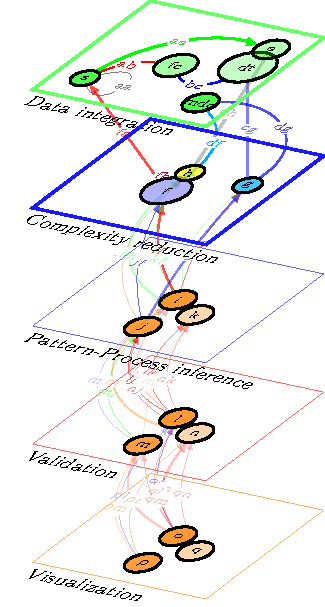
\includegraphics[width=9cm,height=14cm]{Figure1.pdf}\\
\end{center}
\caption{A cartoon of a five layer automated research platform: Data
  Integration, Complexity reduction, Pattern-process inference,
  Validation, and Visualization. Nodes and links represent algorithms
  and interactions between two algorithms, respectively. For example,
  the figure shows five algorithms in the layer Data integration
  ({\bf a}, {\bf b}, {\bf c}, {\bf d}, and {\bf e}). Algorithm {\bf a}
  interacts with algorithm {\bf b} and {\bf e} in the same layer
  (intra-layer connections) and with algorithm {\bf f} from the second
  layer (inter-layer connection), Complexity reduction. The cartoon
  represents many intra- and inter-layer connections to solve a
  problem. The paths can be quantified by many metrics each producing
  a distribution of automated solutions. This distribution can be
  analyzed with the ones used for a specific domain in science, the
  science of science of a domain, to quantify properties as
  robustness, reproducibility and bias of a domain.}
\label{}
\end{figure}
  
\newpage
%The 5 layers described 
\begin{figure}
    %\vspace{-7 in}
\begin{center}
\hspace{-0.5 in}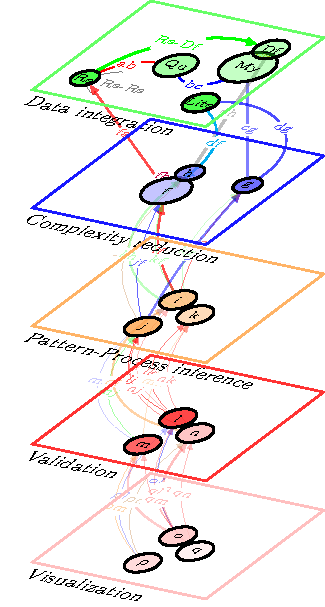
\includegraphics[width=9cm,height=14cm]{Figure2.pdf}\\
\end{center}
\caption{A julia prototype of an automated research platform. Nodes
  and links in each layer represent julia packages and interactions
  between two packages, respectively. The figure shows julia packages
  within each layer. For example, the layer Data integration contains
  the packages "Retriever.jl" ({\bf Re}), "Query.jl" ({\bf Qu}),
  "MySQL.jl" ({\bf My}), "SQlite.jl" ({\bf lite}), and "DataFrames.jl"
  ({\bf df}). }


%Algorithm \bf{a} interacts with algorithm \bf{b} and \bf{e} in the
%same layer (intra-layer connections) and with algorithm \bf{f} from
%the second layer (inter-layer connection), Complexity reduction.

%The cartoon represents many intra- and inter-layer connections to
%solve a problem. The paths can be quantified by many metrics each
%producing a distribution of automated solutions. This distribution can
%be analyzed with the ones used for a specific domain in science, the
%science of science of a domain, to quantify properties as robustness,
%reproducibility and bias of a domain.  }
\label{}
\end{figure}

%\newpage
%\begin{figure}
%\begin{center}
%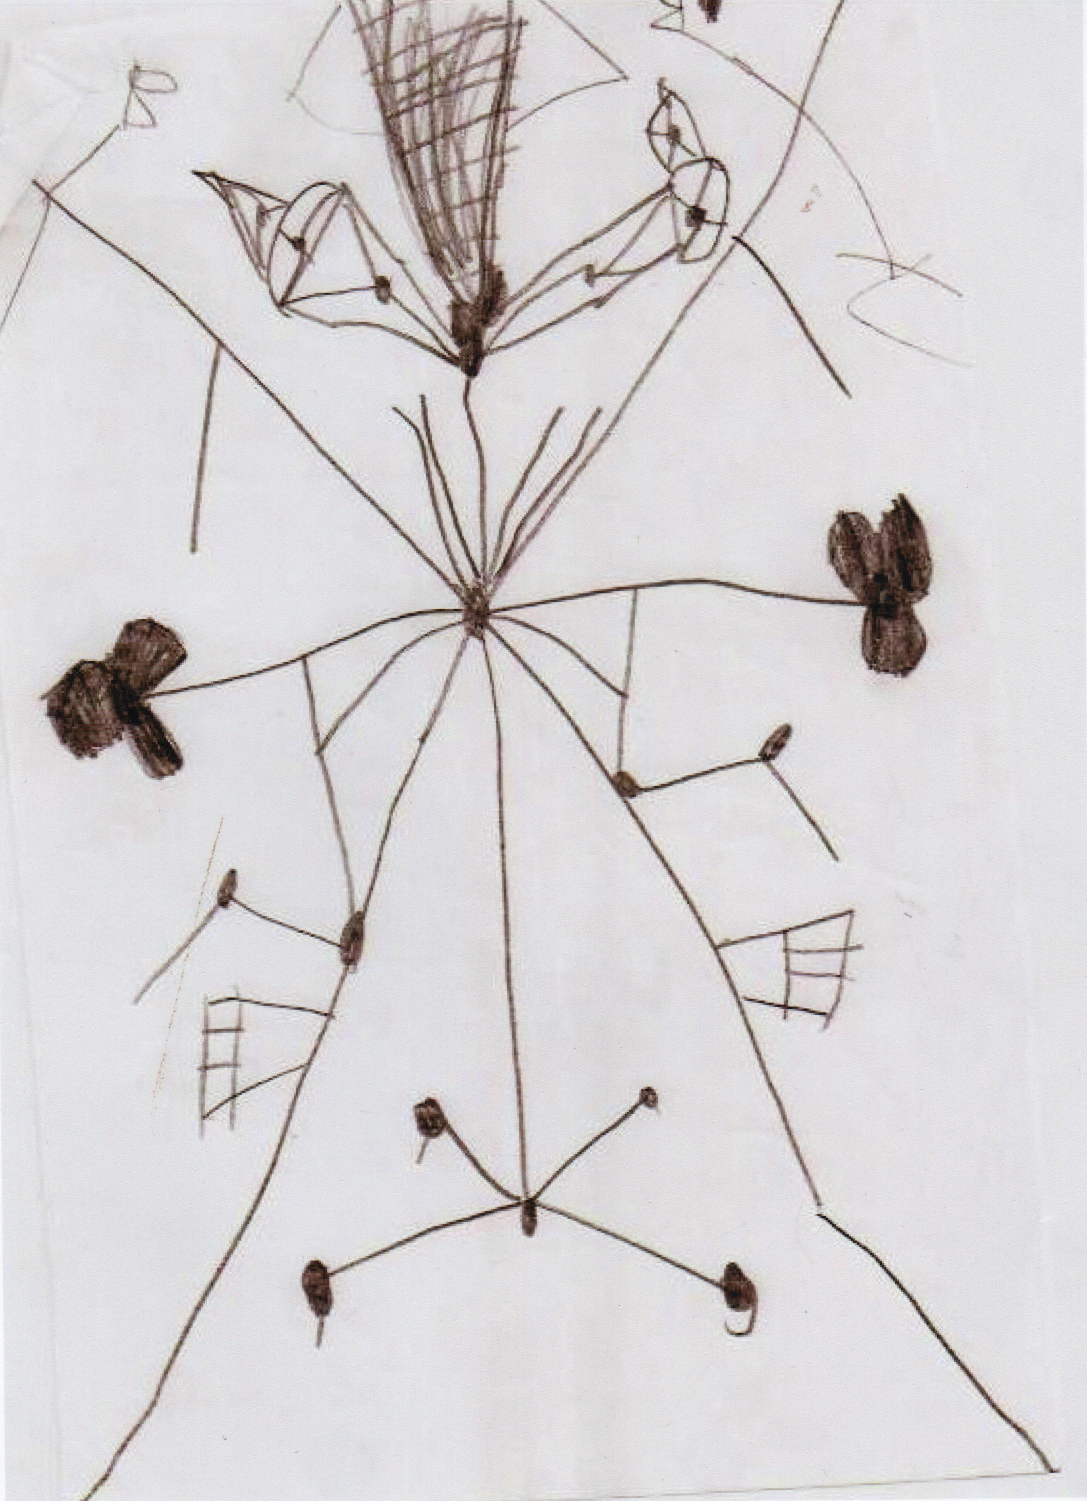
\includegraphics[scale=0.4]{robhootcartoon.pdf}
%\end{center}
%\caption{$\mathcal{ROBHOOT}$} -- An open multilayer platform for data integration, inference and prediction}
%\end{figure}
%\newpage



\newpage

%\begin{figure}
%\vspace{-1 in}
%\begin{center}
%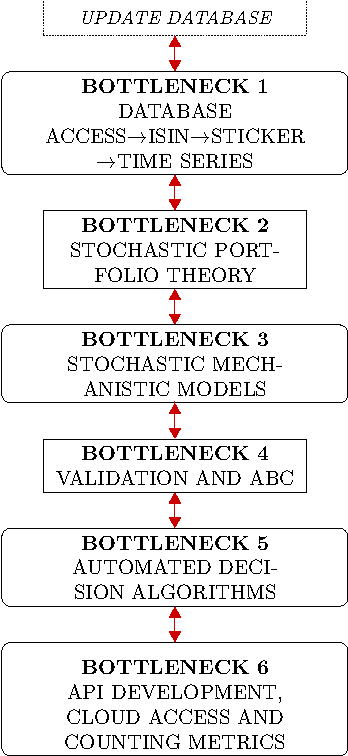
\includegraphics[scale=1.25]{EasyFlowChartBottlenecks.pdf}
%\end{center}
%\caption{Packages graph in $\mathcal{ROBHOOT}$: Visualization: Julia(Tikz and Tikz-network)}
%\end{figure}
%\newpage


\printindex
\end{document}
